\section{解的趋同：对优化器、场景与权重的稳健性检验}\label{sec:converge}

\begin{chapterquestion}
\textbf{本章研究的问题}：解的趋同对优化器、场景与权重的变化是否稳健？
\end{chapterquestion}

可信性分析的三个环节已经完成，但第~\ref{sec:anomaly}~节的异常二（算法间同解）
与异常三（场景间同解）仍然存在。本节用三组对照实验对这两类异常进行量化，
并新增权重敏感性实验。以下对比的目的不是表明"PSO 最优"，
而是将"不同优化器得到相似解"这一现象本身作为证据。

\subsection{对优化算法的稳健性：PSO、GA、DE 结果接近}

在同一 XGBoost 代理上，让 PSO（自适应）、GA、DE、SA 各独立运行 20 次：

\begin{table}[H]
\centering
\caption{四种计算智能算法对比（20 次独立试验，均值$\pm$标准差）}
\begin{tabular}{lrrrr}
\toprule
算法 & 适应度 & 迭代数 & 耗时 (ms) & 收敛率 \\
\midrule
PSO（自适应） & $100.26\pm0.10$ & 28.9 & \textbf{71.8} & \textbf{100\%} \\
遗传算法 (GA) & $\mathbf{100.29}\pm0.12$ & 36.1 & 970.4 & 100\% \\
差分进化 (DE) & $100.27\pm0.10$ & 30.3 & 768.9 & 100\% \\
模拟退火 (SA) & $100.14\pm0.08$ & 441.6 & 239.9 & 0\% \\
\bottomrule
\end{tabular}
\label{tab:ci_comparison}
\end{table}

\begin{figure}[H]
\centering
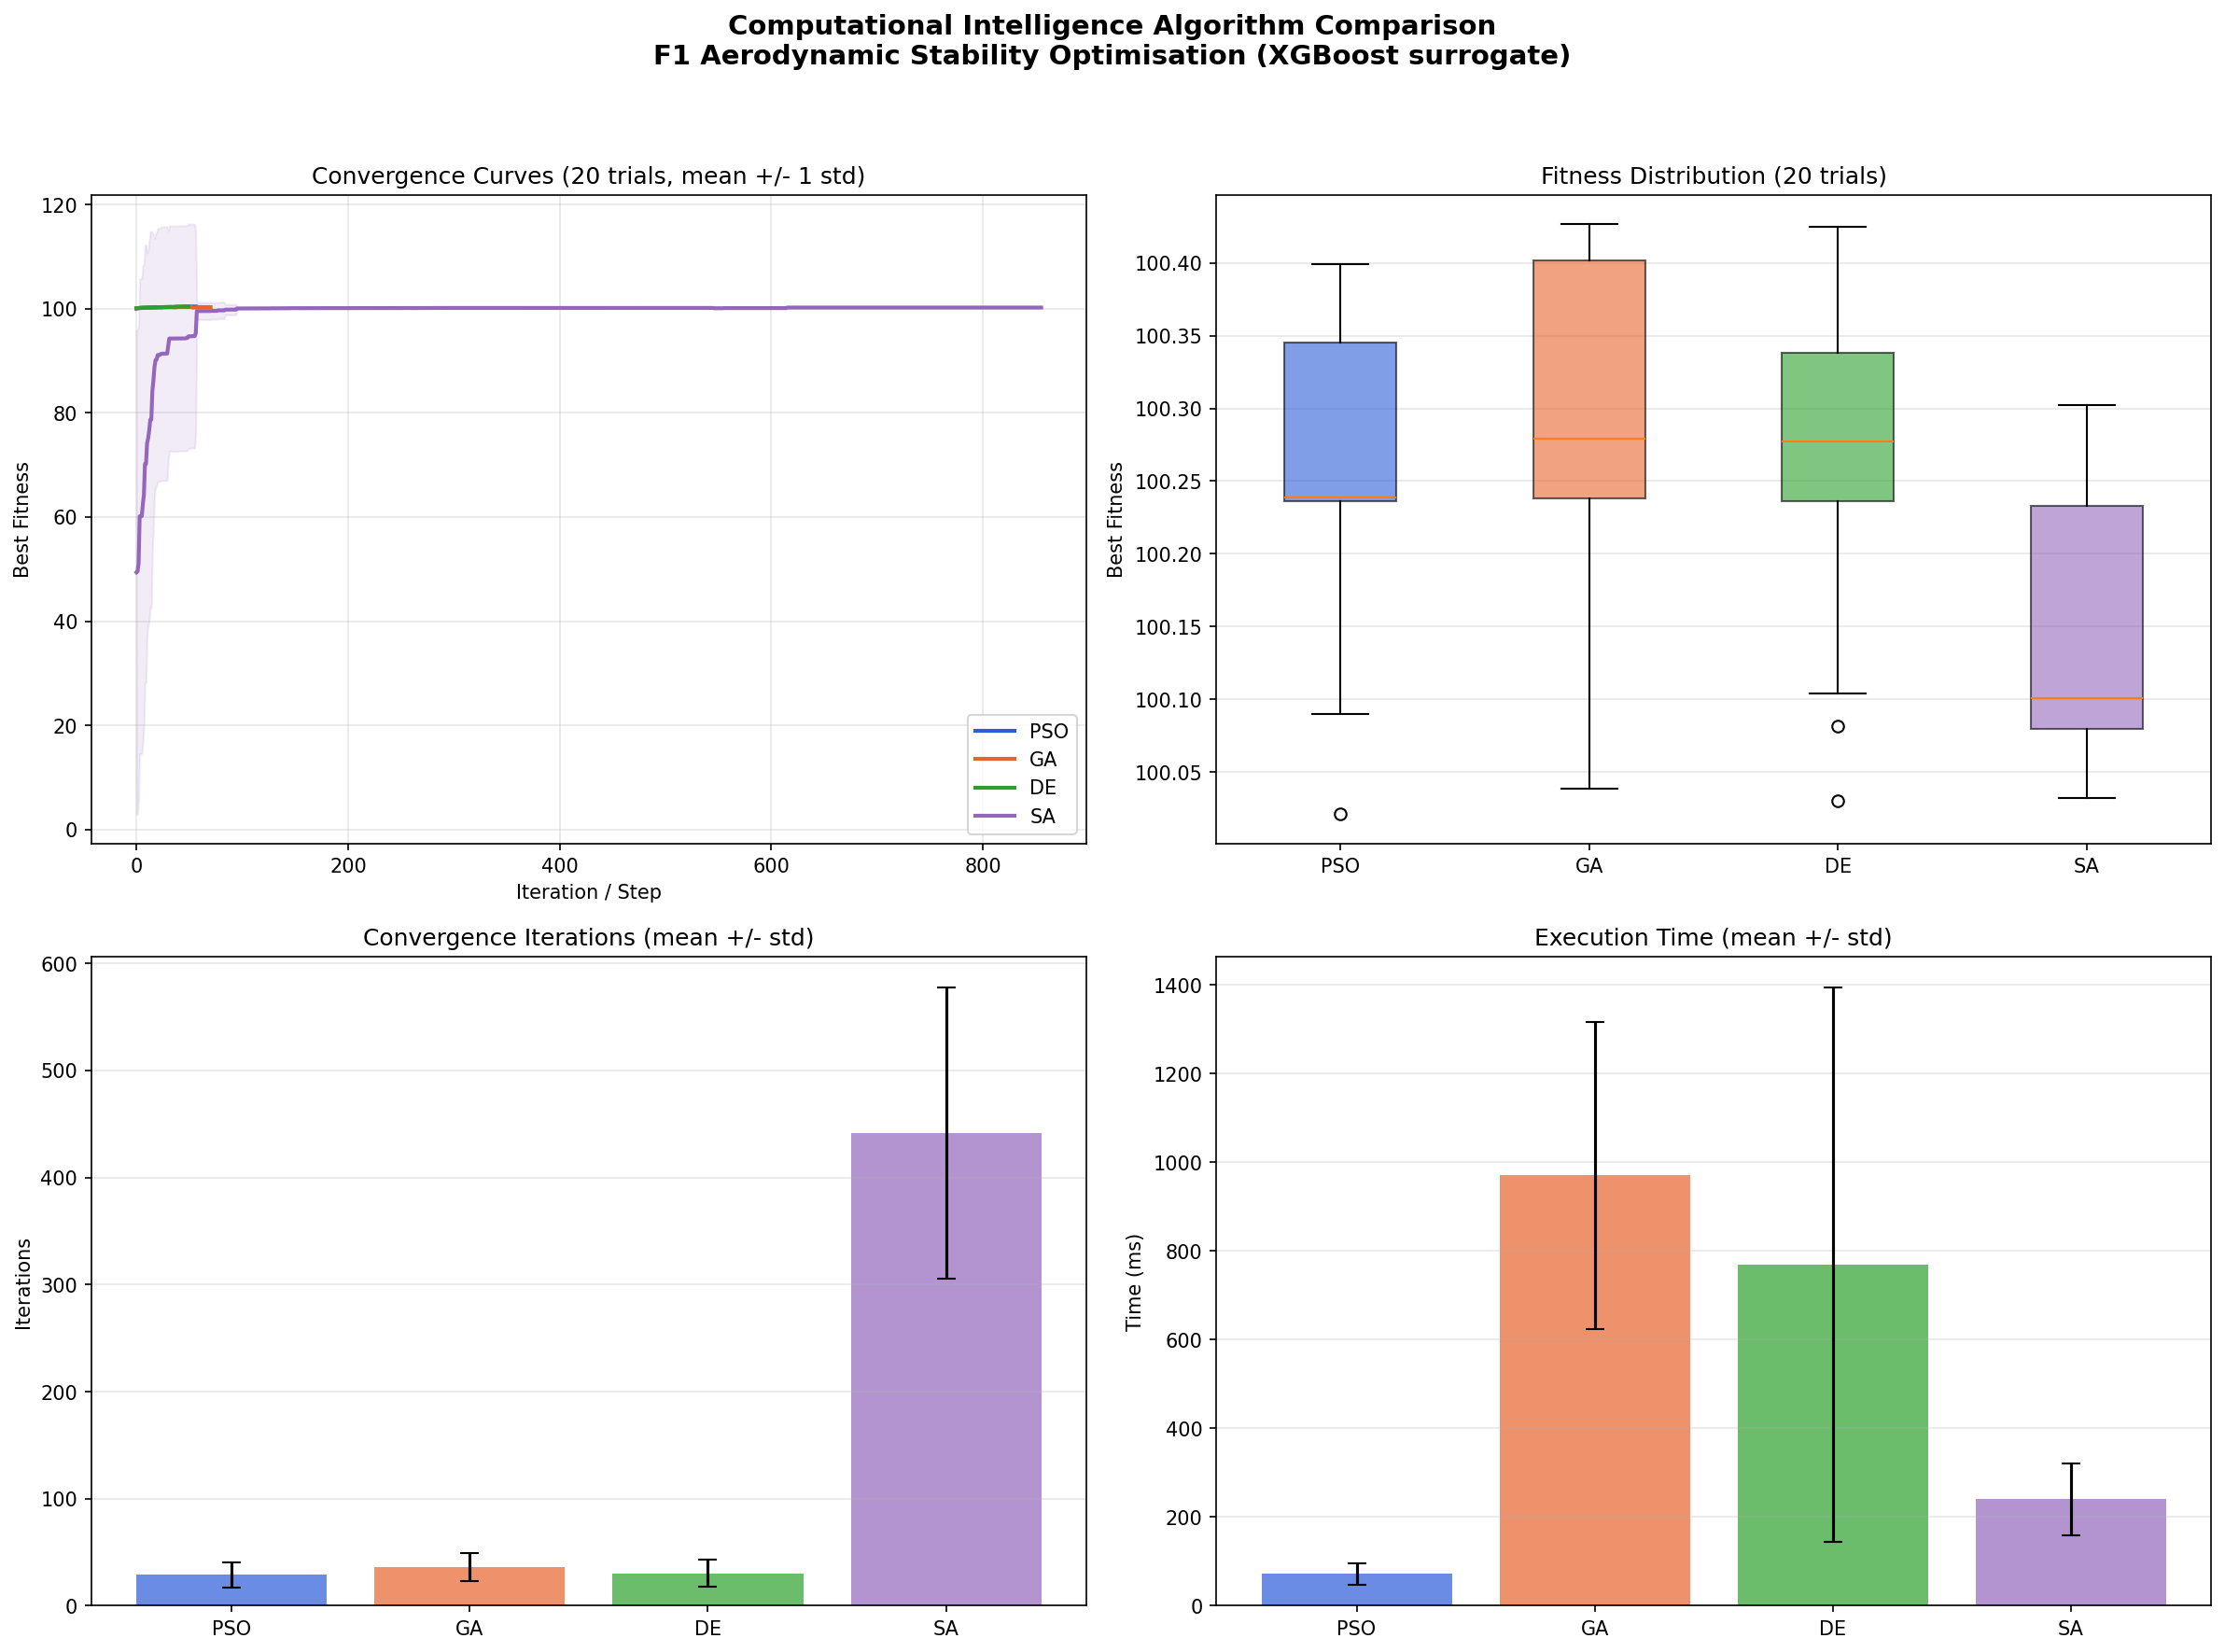
\includegraphics[width=0.92\textwidth]{figures/16_ci_comparison.png}
\caption{四算法对比——收敛曲线、适应度分布、迭代数与耗时}
\label{fig:ci}
\end{figure}

表~\ref{tab:ci_comparison} 表明：
PSO、GA、DE 的最优适应度集中在 $100.14$--$100.29$，\textbf{极差仅 0.15}。
三种搜索机制不同的优化器得到了高度接近的解，
这削弱了"优化器是主要瓶颈"的解释。
PSO 在此并非显著更优，而是在与 GA/DE 解质量接近的前提下耗时最低
（$71.8$ ms，对比 GA $970$ ms、DE $769$ ms），综合效率较好，
且其群体信息共享机制与《计算智能》课程方法论契合，故作为主要优化器。
SA 收敛率为 $0\%$：单点随机游走在近乎平坦的景观上效率较低，
这一现象也与景观平坦的判断一致。

\subsection{对赛道场景的稳健性：四场景解高度趋同}

四组差异较大的赛道工况下运行多目标 PSO（加权标量化，
$F=w_1\,\text{stab}/100+w_2\tilde e-w_3\tilde p-\lambda\sigma$；
需说明这是\emph{加权标量化}而非 NSGA-II 式的种群非支配搜索）：

\begin{table}[H]
\centering
\caption{四场景最优参数汇总——wing 与 drag 高度趋同}
\begin{tabular}{lrrrrrr}
\toprule
场景 & speed & wing & drs & downforce (N) & drag (N) & 复合适应度 \\
\midrule
S1 Monza & 345.0 & 20.1 & 1.0 & 4248.7 & 18.0 & 0.685 \\
S2 Monaco & 300.0 & 20.0 & 0.0 & 4454.2 & 18.0 & 0.894 \\
S3 均衡 & 320.0 & 20.0 & 1.0 & 4411.6 & 18.0 & 0.790 \\
S4 湿地 & 290.0 & 20.0 & 0.0 & 4480.8 & 18.0 & 0.791 \\
\bottomrule
\end{tabular}
\label{tab:scenario_opt}
\end{table}

尽管四场景的权重向量差异显著（S1 偏效率，S4 偏稳定），
\textbf{翼角均约为 $20^\circ$、阻力均为下界 $18$ N}，
场景差异只通过被硬约束固定的速度/DRS 体现。
其中 Monza（DRS 开）与 Monaco（DRS 关）的 drag 完全相同，
表明 DRS 在该代理中边际贡献接近零（SHAP mean$|$value$|$ 仅 $0.01$），
即 DRS 在数据生成器中近乎失效。
复合适应度在 $0.685$--$0.894$ 间有 $>23\%$ 的区分（多目标使部分景观产生区分），
但该区分并未转化为 wing/drag 维度上解的分化。

\subsection{对偏好权重的稳健性（新增实验）}

若场景间同解是因为各场景权重差异不足，
则系统地扫描权重应当能够改变解。为此本文新增权重敏感性实验：
固定一套场景几何（均衡场景），在单纯形上取 \textbf{36 组}差异显著的权重向量
$(w_s,w_e,w_p)$，对每组独立寻优并记录最优解的位移。

\begin{figure}[H]
\centering
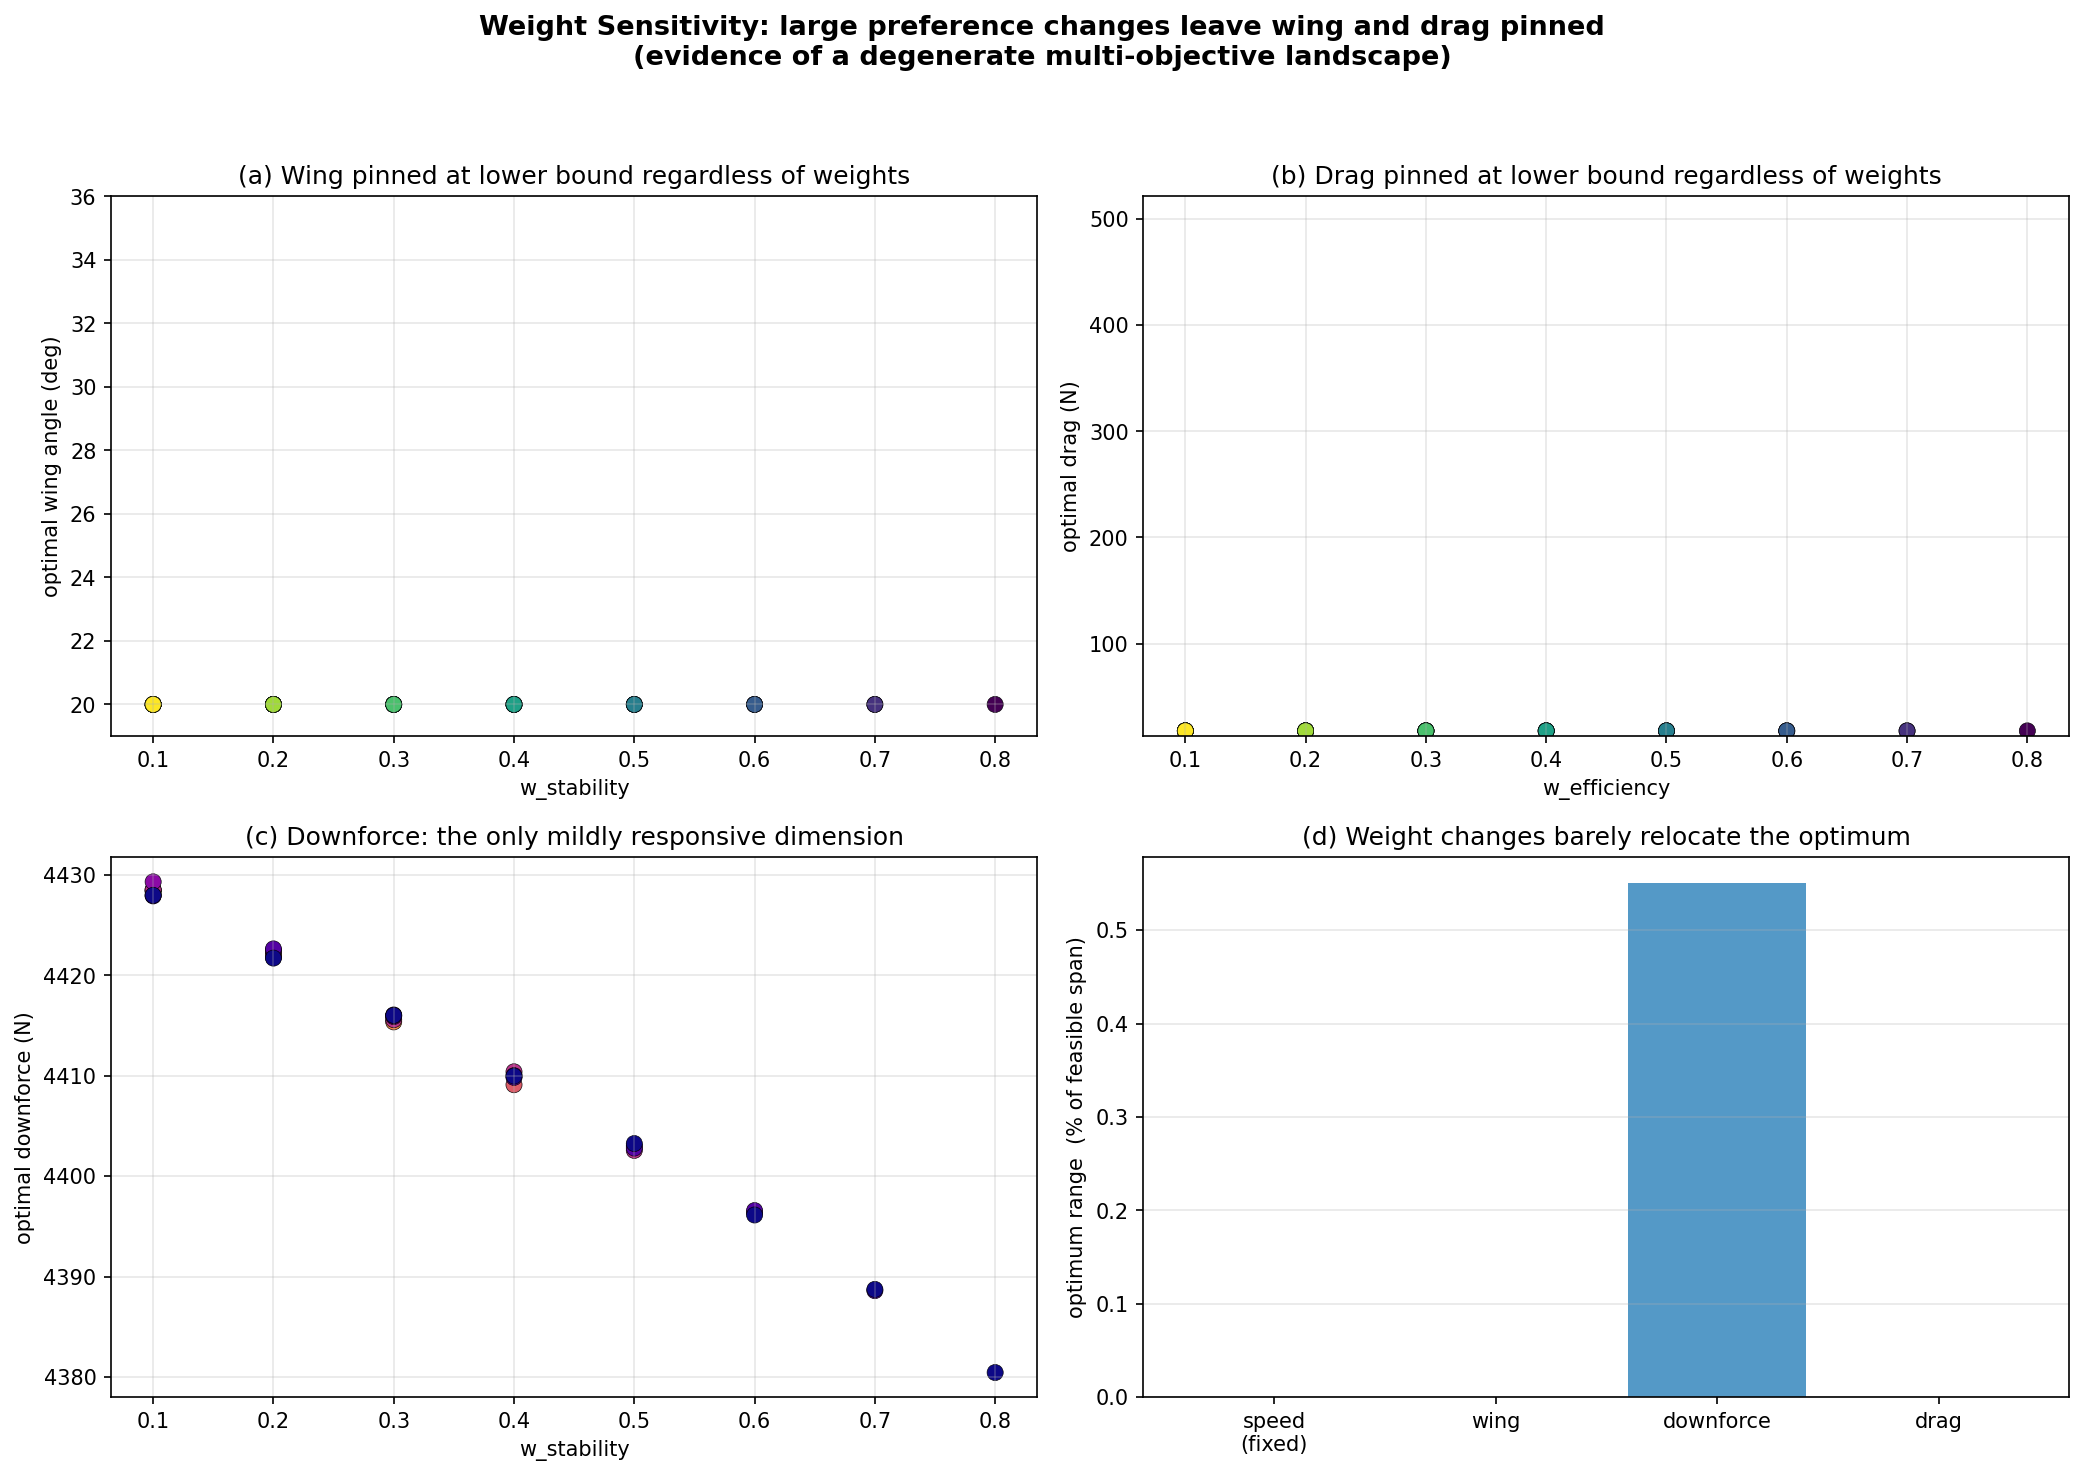
\includegraphics[width=0.95\textwidth]{figures/18_weight_sensitivity.png}
\caption{不同权重向量下最优解的分布}
\label{fig:weight}
\end{figure}

结果显示（图~\ref{fig:weight}）：在全部 36 组权重下，
\textbf{最优翼角与最优阻力的位移均为 0\%}（均位于下界），
唯一略有响应的下压力也仅移动可行范围的 \textbf{0.6\%}。
这进一步支持以下判断：

\begin{chapterquestion}
当差异显著的偏好权重几乎无法改变最优解时，主要影响因素已不在权重设计或优化器搜索能力，
而更可能在于优化景观本身的退化。
\end{chapterquestion}

\subsection{三组对照的综合}

三组对照（优化器、场景、权重）呈现一致趋势：
解的趋同不随优化器、场景或权重而改变，可信性分析也未能消除它。
上述一致趋势与目标函数景观退化的解释一致。
第~\ref{sec:landscape}~节对这一现象进行综合分析。
